\documentclass[10pt]{beamer}
\usepackage[utf8x]{inputenc}
\usepackage{hyperref}
\usepackage{fontawesome}
\usepackage{graphicx}
\usepackage[english,ngerman]{babel}

% ------------------------------------------------------------------------------
% Use the beautiful metropolis beamer template
% ------------------------------------------------------------------------------
\usepackage[T1]{fontenc}
\usepackage{fontawesome}
\usepackage{FiraSans} 
\mode<presentation>
{
  \usetheme[progressbar=foot,numbering=fraction,background=light]{metropolis} 
  \usecolortheme{default} % or try albatross, beaver, crane, ...
  \usefonttheme{default}  % or try serif, structurebold, ...
  \setbeamertemplate{navigation symbols}{}
  \setbeamertemplate{caption}[numbered]
  %\setbeamertemplate{frame footer}{My custom footer}
} 

% ------------------------------------------------------------------------------
% beamer doesn't have texttt defined, but I usually want it anyway
% ------------------------------------------------------------------------------
\let\textttorig\texttt
\renewcommand<>{\texttt}[1]{%
  \only#2{\textttorig{#1}}%
}

% ------------------------------------------------------------------------------
% minted
% ------------------------------------------------------------------------------
\usepackage{minted}


% ------------------------------------------------------------------------------
% tcolorbox / tcblisting
% ------------------------------------------------------------------------------
\usepackage{xcolor}
\definecolor{codecolor}{HTML}{FFC300}

\usepackage{tcolorbox}
\tcbuselibrary{most,listingsutf8,minted}

\tcbset{tcbox width=auto,left=1mm,top=1mm,bottom=1mm,
right=1mm,boxsep=1mm,middle=1pt}

\newtcblisting{myr}[1]{colback=codecolor!5,colframe=codecolor!80!black,listing only, 
minted options={numbers=left, style=tcblatex,fontsize=\tiny,breaklines,autogobble,linenos,numbersep=3mm},
left=5mm,enhanced,
title=#1, fonttitle=\bfseries,
listing engine=minted,minted language=r}


% ------------------------------------------------------------------------------
% Listings
% ------------------------------------------------------------------------------
\definecolor{mygreen}{HTML}{37980D}
\definecolor{myblue}{HTML}{0D089F}
\definecolor{myred}{HTML}{98290D}

\usepackage{listings}

% the following is optional to configure custom highlighting
\lstdefinelanguage{XML}
{
  morestring=[b]",
  morecomment=[s]{<!--}{-->},
  morestring=[s]{>}{<},
  morekeywords={ref,xmlns,version,type,canonicalRef,metr,real,target}% list your attributes here
}

\lstdefinestyle{myxml}{
language=XML,
showspaces=false,
showtabs=false,
basicstyle=\ttfamily,
columns=fullflexible,
breaklines=true,
showstringspaces=false,
breakatwhitespace=true,
escapeinside={(*@}{@*)},
basicstyle=\color{mygreen}\ttfamily,%\footnotesize,
stringstyle=\color{myred},
commentstyle=\color{myblue}\upshape,
keywordstyle=\color{myblue}\bfseries,
}


% ------------------------------------------------------------------------------
% The Document
% ------------------------------------------------------------------------------
\title{Reinforcement Learning and Robotics -\\ Opportunities and Challenges }
\author{Sarah Keren}
\date{June 2020}

\begin{document}

\maketitle

\begin{frame}{Objectives}
\begin{itemize}
    \item Reinforcement learning (RL) has been very successful in many artificial environments and some real-world domains
    \begin{itemize}
        \item Playing Go, Chess, Poker
        \item Make a humanoid robot walk
        \item Managing an investment portfolio
    \end{itemize}
    
    \bigskip
    
    \item What are the benefits and limitations of using RL for in robotics ?
\end{itemize}
\end{frame}

\begin{frame}{A little bit about me}
\begin{itemize}
    \item I am a post-doc at the Center for Research on Computation and Society @Harvard, working with Prof. David Parkes and Prof. Barbara Grosz.
    \item The overall objective of my research is to use principled automated design to promote effective multi-agent collaboration and to enhance the way robots and machines interact with humans.
    \item My background is in automated planning and model based reasoning. 
    \item Example frameworks:
    \begin{itemize}
    \item Goal Recongition Design
    \item Equi-Reward Utility Maximizing Design
    \item Information Shaping
    \end{itemize}
\end{itemize}
\end{frame}

\begin{frame}{My current projects:}
\begin{enumerate}

    \item Economic Hierarchical Reinforcement Learning for Efficient Planning for Robots (and other AI agents) 
    \item Reinforcement Learning Design
    \item Interpretability of Reinforcement Learning results
\end{enumerate}

\begin{figure}
	\centering
	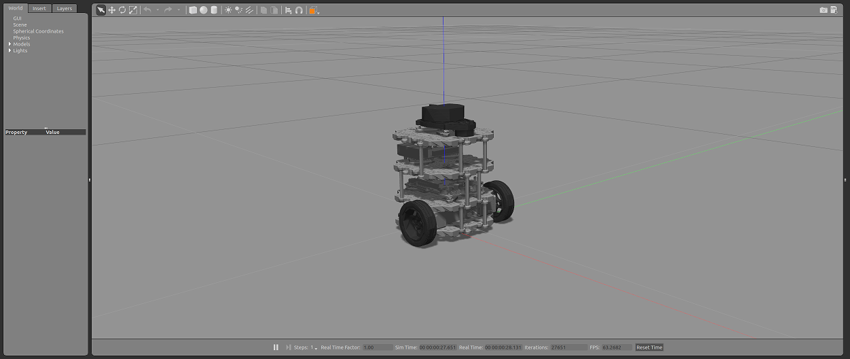
\includegraphics[scale=0.35]{images/turtlebot3_empty_world}
\end{figure}

\end{frame}


\section{(A very brief) Introduction to Reinforcement Learning}
\begin{frame}{What is Reinforcement Learning (RL) ?}


\begin{figure}
	\centering
	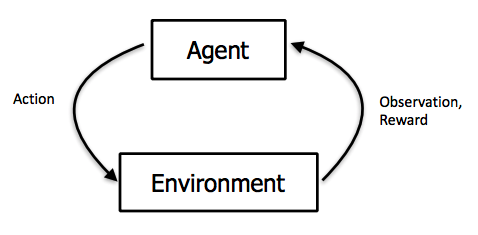
\includegraphics[scale=0.35]{images/RL}
\end{figure}


\end{frame}
\begin{frame}{What is Reinforcement Learning (RL) ?}
\begin{itemize}
    \item RL involves an agent, a set of states  and a set  of actions per state.
    \item By performing an action, the agent transitions from state to state.
    \item Executing an action in a specific state provides the agent with a reward (a numerical score).
    \item The goal of the agent is to maximize its total reward. It does this by adding the maximum reward attainable from future states to the reward for achieving its current state, effectively influencing the current action by the potential future reward.
    \item  This potential reward is (typically) a weighted sum of the expected values of the rewards of all future steps starting from the current state.
 \end{itemize}
 Taken from wikipedia
\end{frame}
 
 \begin{frame}{What is Reinforcement Learning (RL) ?}
 
 The process of Reinforcement Learning involves these steps:
 \begin{itemize}
     \item Observation of the environment
     \item Deciding how to act using some strategy
     \item Acting accordingly
    \item Receiving a reward or penalty
    \item Learning from the experiences and refining our strategy
    \item Iterating until an optimal strategy is found
 \end{itemize}
 
 Let's see an example

 \end{frame}
 
 
 \begin{frame}{What is Reinforcement Learning (RL) ?}
 
 Two fundamental problems in sequential decision making
 \begin{itemize}
     \item {\bf Reinforcement Learning:}
The environment is initially unknown
The agent interacts with the environment
The agent improves its policy
\item {\bf Planning:}
A model of the environment is known
The agent performs computations with its model (without any
external interaction)
The agent improves its policy
a.k.a. deliberation, reasoning, introspection, pondering,
thought, search
 \end{itemize}


\end{frame}

\begin{frame}{Reinforcement Learning (RL) vs. Machine Learning (ML)}
   
What makes reinforcement learning different from other machine
learning paradigms?
\begin{itemize}
    \item There is no supervisor, only a reward signal
    \item Feedback is delayed, not instantaneous
    \item Time really matters (sequential, non i.i.d data)
Agent’s actions affect the subsequent reward it receives
\end{itemize}



\begin{figure}
	\centering
	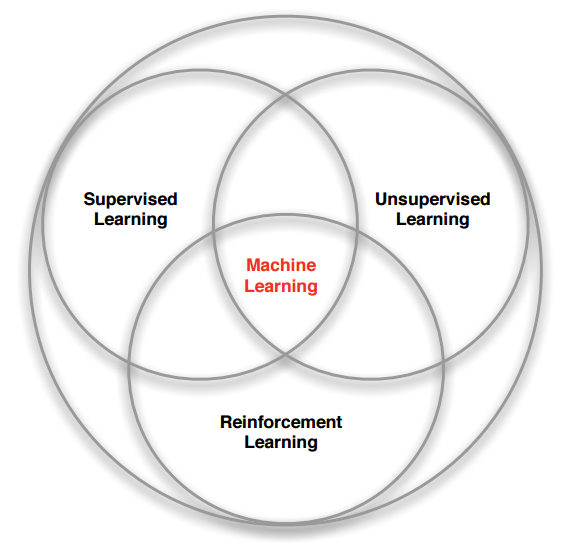
\includegraphics[scale=0.3]{images/RL-ml.png}
	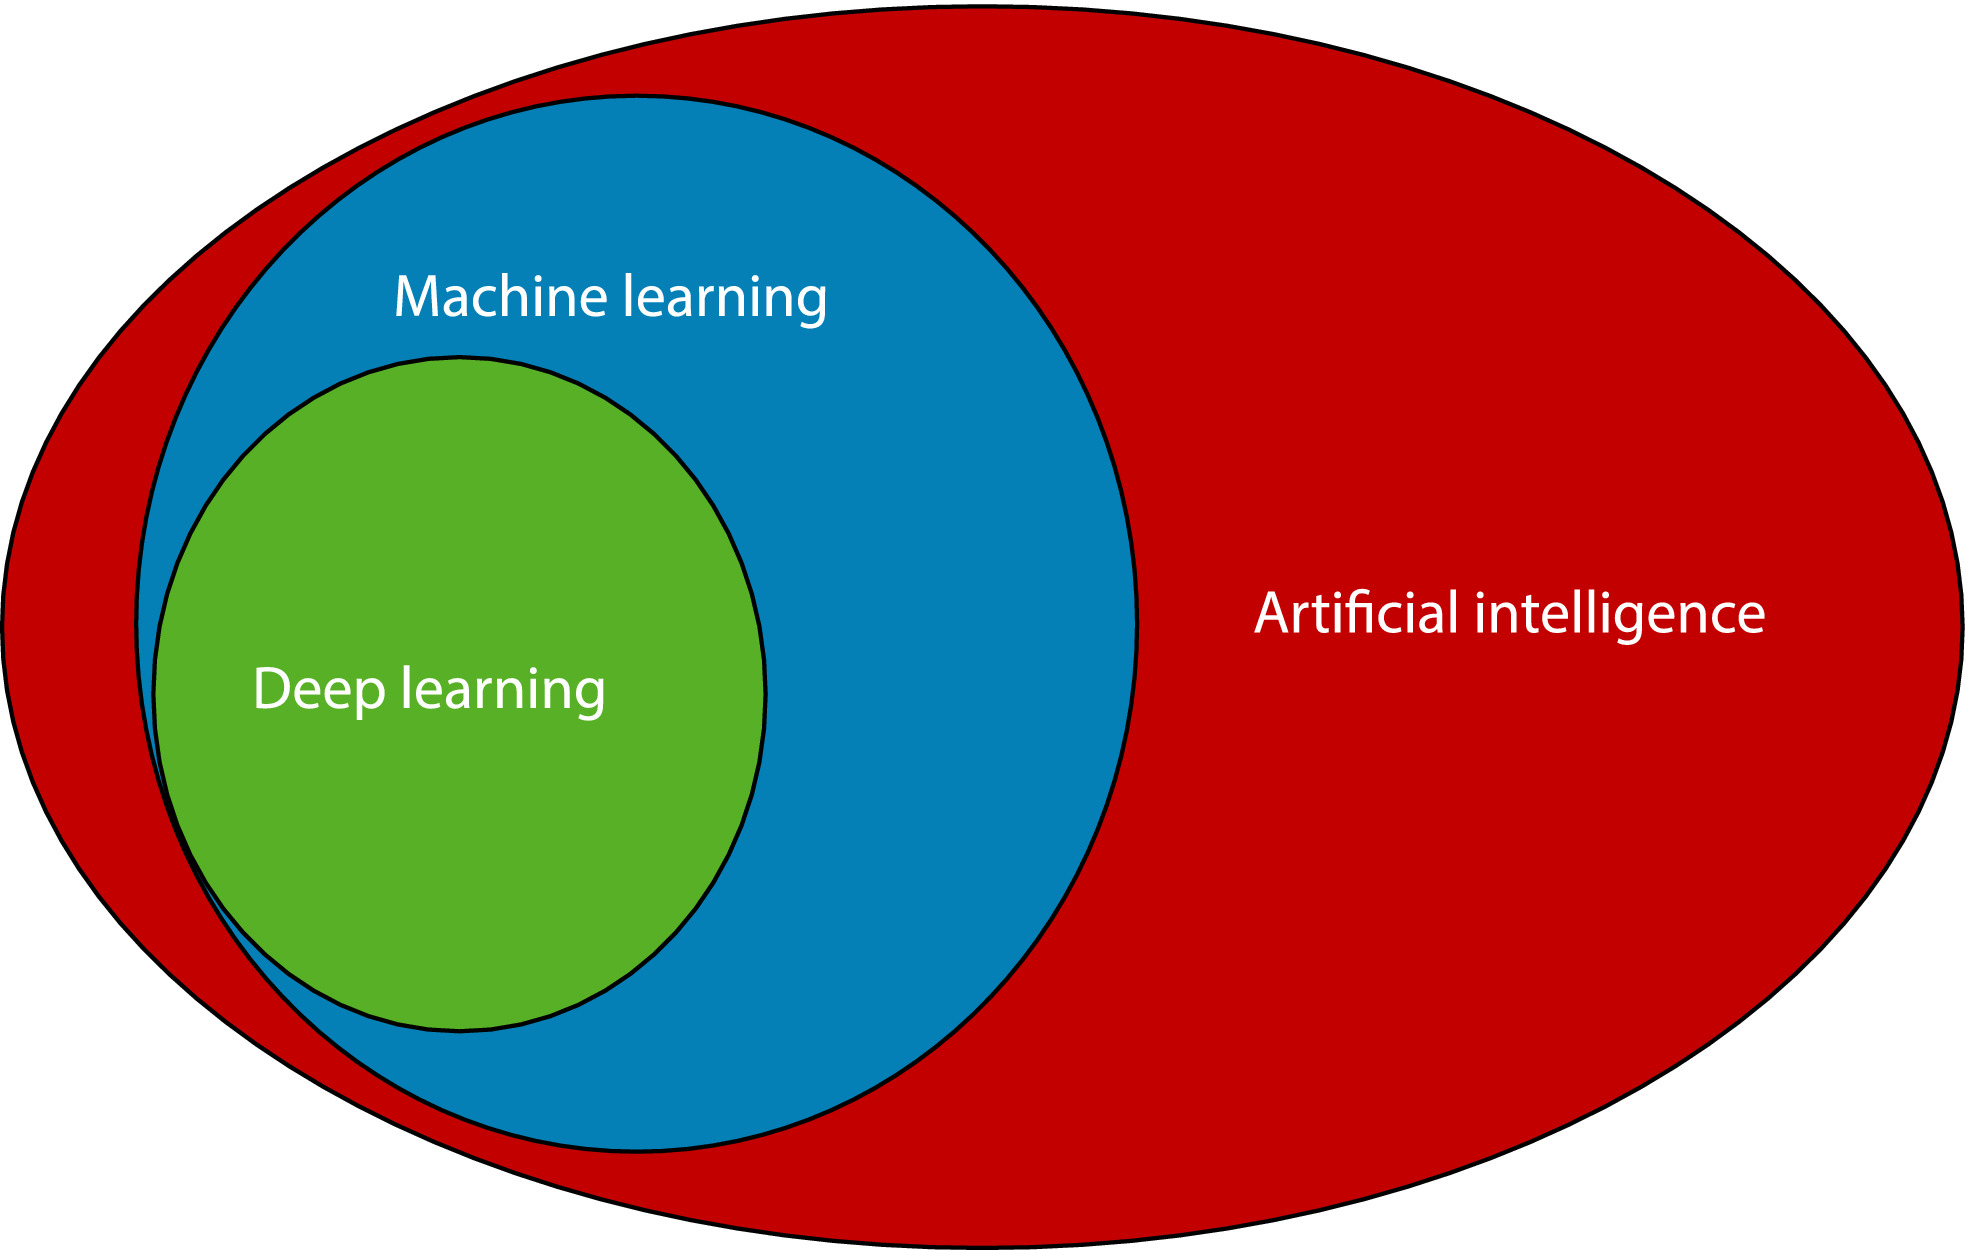
\includegraphics[scale=0.55]{images/AI}
\end{figure}

\end{frame}

\begin{frame}{Model: Markov Decision Process}

A {\bf Markov Decision Process}(MDP) is a tuple $\langle \mathcal{S}, \mathcal{A}, \mathcal{P}, \mathcal{R}, \gamma\rangle$ where
\begin{itemize}
    \item $\mathcal{S}$ is a finite set of states
    \item $\mathcal{A}$ is a finite set of actions
    \item $\mathcal{P}$ is a state transition probability matrix
    $\mathcal{P}^{a}_{s,s'}= \mathbb{P}[S_{t+1}=s'|S_t=s, A_t=a]$
    \item $\mathcal{R}$ is a reward function, $\mathcal{R}^a_s = \mathbb{E}[R_{t+1} | S_t = s, A_t = a]$, and
    \item $\gamma$ is a discount factor $\gamma \in [0, 1]$ 

\end{itemize}

The Markov property: 
“The future is independent of the past given the present”

\bigskip

What is the MDP representation of the example we saw ?

\end{frame}

\begin{frame}{Model: Markov Decision Process}

A {\bf policy} $\pi$ is a distribution over actions given states,
$$\pi(a|s) = \mathbb{P}[A_t = a | S_t = s]$$

The {\bf state-value function} $v_{\pi}(s)$ of an MDP is the expected return starting from state $s$, and then following policy $\pi$

$$v_{\pi} (s) = \mathbb{E}_{\pi}[G_t | S_t = s]$$

The {\bf action-value function} $q_{\pi}(s, a)$ is the expected return
starting from state $s$, taking action $a$, and then following policy $\pi$
$$q_{\pi}(s, a) = \mathbb{E}_{\pi} [G_t | S_t = s, A_t = a]$$

\end{frame}


\begin{frame}{Model: Extensions}
\begin{itemize}
    \item Infinite and continuous MDPs
    \item Partially observable MDPs
    \item Undiscounted, average reward MDPs
\end{itemize}


\end{frame}

\begin{frame}{Solution Approaches: MDP}
Many iterative solution methods
\begin{itemize}
    \item Value Iteration
    \item Policy Iteration
    \item Q-learning
\end{itemize}

\end{frame}

\begin{frame}{Solution Approaches: RL}

In RL there's a tradeoff between {\bf exploration} (choosing a random action) and {\bf exploitation} (choosing actions based on already learned values).


\begin{figure}
	\centering
	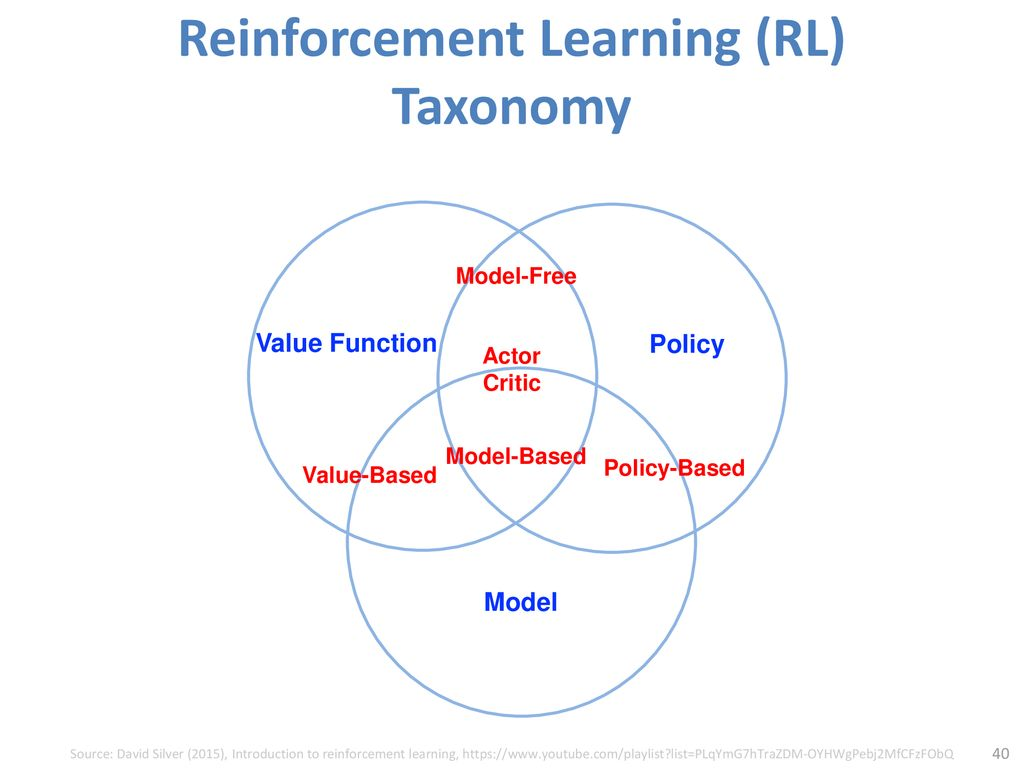
\includegraphics[scale=0.55]{images/RL-Tax.jpg}
\end{figure}

By David Silver
\end{frame}

\begin{frame}{Three general solution approaches}

\begin{itemize}
    \item {\bf Action value methods}:  Learning estimations of values of state-action pairs\\
    For example: \\
    \begin{itemize}
        \item  Q learning (the rl equivalent to value-iteration in MDPs)
        \item UCB approaches
    \end{itemize}

     \item {\bf Gradient based methods:}
     Learning a numerical preference of each action which determines its probability of being executed 
     For example:\\
     \begin{itemize}
         \item  Stochastic Gradient Ascent (the rl equivalent to policy iteration)
     \end{itemize}


     \item {\bf Actor-critic methods:}
     combines the value optimization and policy optimization approaches.\\


\end{itemize}    

Deep learning versions of all approaches

\end{frame}


\begin{frame}{Multi-Agent Markov Decision Process - Markov Games}

A {\bf MARL Markov game} is defined by the tuple $\langle \mathcal{S}, \mathcal{A}, \mathcal{P}, \mathcal{R}, \gamma\rangle$ where
\begin{itemize}
    \item $\mathcal{S}$ is a finite set of states
    \item $\mathcal{A} = \{A^i\}_{i=1}^{n}$  is a collection of action sets $A^i$ , one for each
agent in the environment. At each timestep $t$, each agent $i$ chooses an action $a^i_t \in A^i$. The actions of all $N$ agents are combined to form a joint action $a_t = [a^0_t, \dots, a^N_t]$, which produces a transition in the environment $p(s_{t+1}|a_t,s_t)$, according to the state transition distribution $\mathcal{P}$,
    \item $\mathcal{R} = \{R^i\}_{i=1}^{n}$ is a collected of rewards functions $R^i$ defining the reward $r^i(a_t,s_t)$ each agent receives when the joint action $a_t$ is performed at state $s_t$,
    \item $\gamma$ is a discount factor $\gamma \in [0, 1]$.
\end{itemize}

In pratially observable environments the $i$th agent can only view a portion of the true state, $s^i_t$.

Typically, each agent seeks to maximize its own total expected discounted future reward %$\Sigma^{\infty}_{i=0}\gamma^i r^k_{}t+1$



\end{frame}


\section{(A very brief) Introduction to Task and Motion Planning for Robotics}

\begin{frame}{Challenges of planning for robots}
\begin{itemize}
    \item As robots become more physically robust and capable of sophisticated sensing, navigation, and manipulation they need to accomplish tasks if increasing complexity.
   \item {\bf Curse-of- dimensionality} - complexity of finding task plans derives from very long time horizons, a large numbers of objects and many ‘degrees of freedom’ of robot configurations to be considered and manipulated
   \item In a 2D world with $5$ objects with only $10$ sampled points along each axis and considering only Manhattan paths for estimating path distances, $10^{11}$ facts are required, resulting in problem instances that are too large to solve efficiently.
\end{itemize}

A common approach: hierarchical approach to planning
\end{frame}

\begin{frame}{Task and motion (path) planning}
\begin{itemize}
    \item Task planners can reason over very large sets of states by manipulating partial descriptions, while geometric (motion) planners operate on completely detailed specifications of world states.
    \item 
A task planner could decide that the living room needs to be traversed, regardless of the detailed arrangement of its furniture. 
    \item 
Motion planners deal beautifully with geometry, but not with non-physical aspects of the domain; they can plan how to get to the phone but not decide that a phone call needs to be made.

\end{itemize}


\end{frame}


\begin{frame}{Task and motion (path) planning}
\begin{figure}
	\centering
	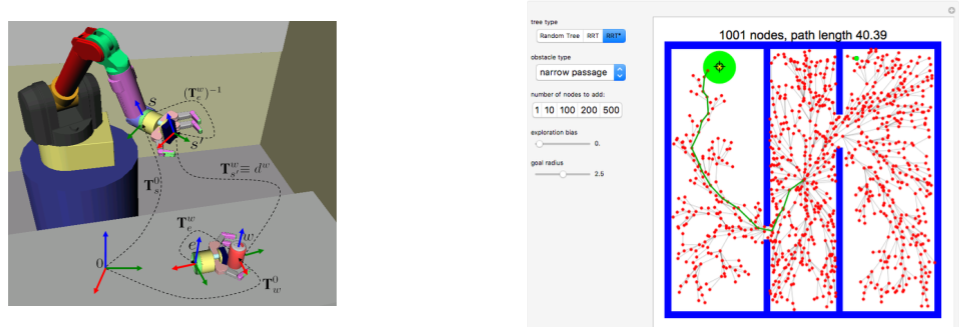
\includegraphics[scale=0.35]{images/task-motion.png}
\end{figure}

Motion planning is not task planning at a higher level of granularity
\end{frame}

\begin{frame}{Task and motion (path) planning}
\begin{figure}
	\centering
	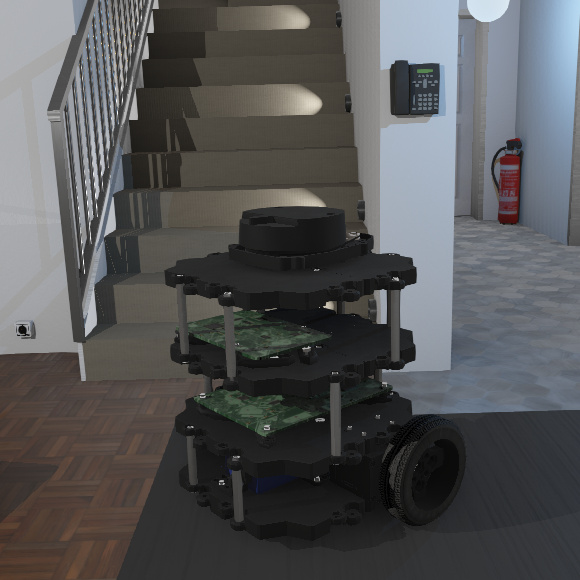
\includegraphics[scale=0.35]{images/turtlebot3.jpg}
\end{figure}

\end{frame}

\section{RL and Robotics}

\begin{frame}{Examples}
A mobile robot decides whether it should enter a new room in search of more trash
to collect or start trying to find its way back to its battery recharging station. It
makes its decision based on the current charge level of its battery and how quickly
and easily it has been able to find the recharger in the past.\\

Sutton and Barto 2018
\end{frame}
\begin{frame}{Examples}


A Pick-and-Place Robot can use RL learn to
control the motion of its arm in a repetitive pick-and-place task. If we want to learn movements that are fast and smooth, the learning agent will have to control the motors
directly and have low-latency information about the current positions and velocities of the
mechanical linkages. The actions might be the voltages applied to each motor
at each joint, and the states might be the latest readings of joint angles and velocities.
The reward might be +1 for each object successfully picked up and placed. To encourage
smooth movements, on each time step a small, negative reward can be given as a function
of the moment-to-moment “jerkiness” of the motion

Sutton and Barto 2018
\end{frame}



\begin{frame}{The kind of papers we will read}
    \begin{itemize}
    \item Multi-agent RL
    \item Task and motion planning for robots
    \item Multi-agent systems
    \end{itemize}
    
    
\end{frame}

\begin{frame}{What we will focus on}
\begin{itemize}
    \item How is RL used for task and motion planning for robotics?
    \item When is RL the best approach ? When is it not ?
    
\end{itemize}

\end{frame}

\begin{frame}{Spoiler}

``So if you look at the issues, you can see that while RL may be a good match with a video games, it’s not as good a fit with a robot operating in the real world.  Model based planning can preserve some of the ideas of RL (to handle incomplete models, exploration), but can also be safer and more efficient. My philosophy is to give complex AI systems all the knowledge we can encode efficiently - instead of learning from scratch - and then use learning to improve them."\\


A leading AI researcher



\end{frame}


\begin{frame}{Presentation Structure}
\begin{itemize}
    \item Motivation
    \item Key contribution
    \item Background and related work
    \item Model and problem statement (input and output)
    \item Approach (algorithmic approach applied)
    \item Evaluation
    \item Conclusion
    \end{itemize}
\begin{figure}
	\centering
	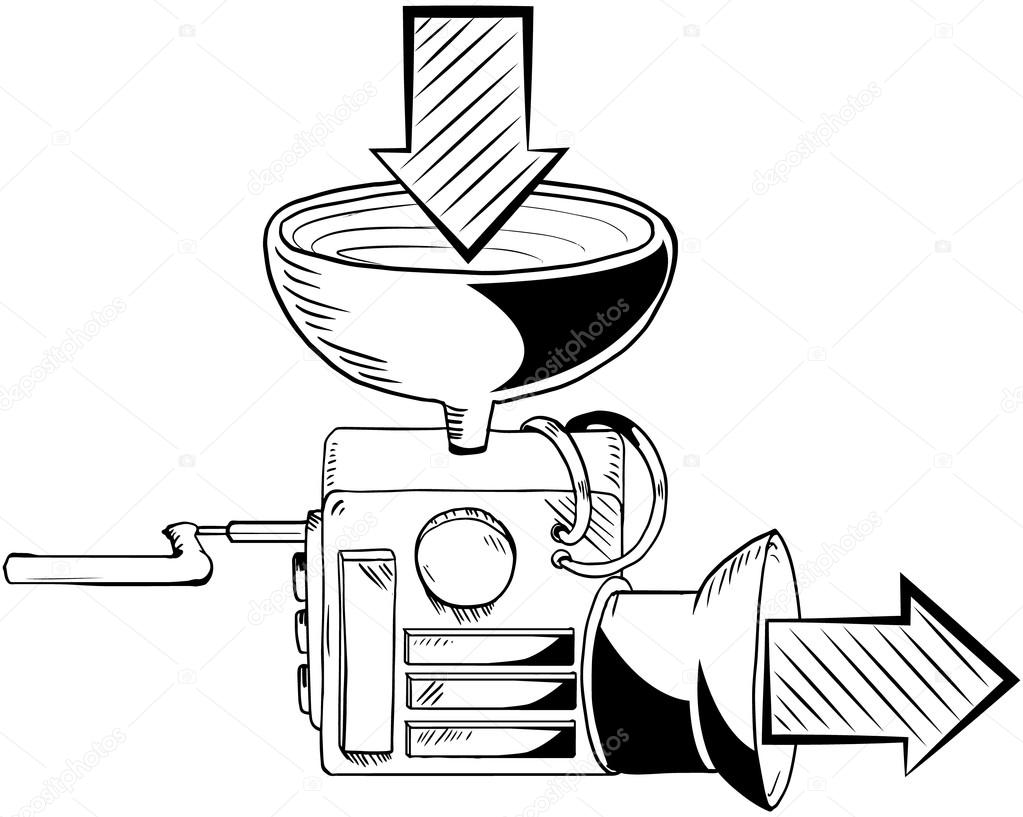
\includegraphics[scale=0.15]{images/machine}
\end{figure}


\end{frame}

\section{RL domains}

\begin{frame}{OpenAI Taxi domain- Sarah}

There are 4 locations (labeled by different letters) and the task involves picking up the passenger at one location and drop him off in another. 


\begin{figure}
	\centering
	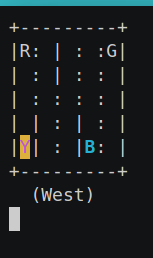
\includegraphics[scale=0.35]{images/taxi}
\end{figure}

https://gym.openai.com/envs/Taxi-v3/
\end{frame}



\begin{frame}{OpenAI Taxi domain: model}

A {\bf Markov Decision Process}(MDP) $\langle \mathcal{S}, \mathcal{A}, \mathcal{P}, \mathcal{R}, \rangle$ where
\begin{itemize}
    \item a state represents the taxi location (taxi row and taxi column) the passenger location and the destination index.
    \item the set of actions the taxi can perform  include moving south, north, east and west as well as passenger pickup and dropoff.
    \item the transition function is deterministic, so the new state is the intended state if the action is legal, and otherwise the agent stays in place, and
    \item the reward function assigns +20 points for a successful dropoff, -1 point for every timestep, and -10 point penalty for illegal pick-up and drop-off actions.
    
\end{itemize}
\end{frame}






\begin{comment}

\section{TO DELETE}

\begin{frame}[fragile,allowframebreaks]{Intro}
When I thought about it, I realized there are actually so many ways of displaying code using LaTeX packages. So I'll start with the most basic and then go on to the more advanced ones ;)
\framebreak

\begin{columns}[T,onlytextwidth]
\column{0.25\textwidth}
\metroset{block=fill}
\begin{exampleblock}{texttt}
\begin{verbatim}
\texttt{}
\end{verbatim}
\end{exampleblock}
\column{0.7\textwidth}
\footnotesize
This one isn't a verbatim way to express code, but it will change the font to typewriter, so it 'looks like code'. However, in these short bits of code, you will have to use escape sequences for reserved characters.

I make massive use of \texttt{} when 'talking' about code or, you know, writing explanatory text sequences. It is especially useful for bits of code where there is no excessive (or none at all) use of escape sequences. Then it is a really handy way to quickly typeset code. Once you have lots of reserved characters, you might be better of just using this next one.
\end{columns}
\framebreak

\begin{columns}[T,onlytextwidth]
\column{0.35\textwidth}
\metroset{block=fill}
\begin{exampleblock}{The verbatim environment}
\texttt{\\begin\{verbatim\}}
    code goes here
\texttt{\\end\{verbatim\}}
\end{exampleblock}
\column{0.6\textwidth}
\footnotesize
\alert{This one really is a staple} and pretty failsafe, but also doesn't have code highlighting which you might want in most cases, apart from very short bits of code where highlighting isn't important.

You can use verbatim as an environment for multiple lines of code which appear like a quote as a separate block in your text. In other cases, where you just want \texttt{} but without having to escape reserved characters, you might want to use the \verb|some code| command. You can use any characters as delimiters to denote beginng and end of code. So it can also be \verb+test+. The idea is that you can choose one which you will not need inside the code, as not to 'confuse' the enviroment.
\end{columns}
\end{frame}

\begin{frame}{Bugs}
\begin{enumerate}
    \item listing all the bugs
    \item oops, this already is one of the main bugs:
    \begin{itemize}
        \item If you were to use the \texttt{enumitem} package
        \item you would get a fatal error
        \item but no output
        \item due to package conflicts
    \end{itemize}
\end{enumerate}
\end{frame}

\section{Tcblisting}

\begin{frame}[fragile]{Tcblisting}
The code is quite tiny because I set the font size to very small in the definition of the little \texttt{myr} 
\begin{myr}{Load files}
# text <- readLines(file.choose())
filePath <- "http://www.link.com/a_text.txt"
text <- readLines(filePath)
\end{myr}
\end{frame}

\section{lstlisting}

\begin{frame}[fragile]{Using Code Listings}
\begin{lstlisting}[language=R]
my_vector <- c("testing","vectors")
my_vector # a test
\end{lstlisting}
\end{frame}

\begin{frame}[fragile]{Using Code Listings II}
This time with caption but without code highlighting.
\begin{lstlisting}[caption={Hello World! in C}]
int main()
{
    printf("Hello World!");
    return 0;
}
\end{lstlisting}
\end{frame}

\begin{frame}[fragile]{Code highlighting with listings}
\begin{lstlisting}[language=Python, caption={A demonstration}]
import numpy as np
\end{lstlisting}

You can also use the inline shorthand for small snippets: \lstinline[language=C]!while{$a || $b}!

\end{frame}

\begin{frame}{List of listings}
    %\lstlistoflistings
    
    Well, this is how it's supposed to be, but sadly, using sections inside frames will add up to this result. -- So you can't use this list of listings here.
\end{frame}



\begin{frame}[fragile]{Importing listing from file}
\lstset{style=myxml} % now we activate the custom style
%\lstinputlisting[language=XML]{my_test.xml}

This will only be in colour if you use the settings.
\end{frame}

\begin{frame}[fragile]{Using Knitr}
<<>>=
# Create sequence
my_sequence = 1:5
 
# use summary function to display stats
summary(my_sequence)
 
@

Then output values inside the text: \Sexpr{my_sequence}.
\end{frame}

\begin{frame}[fragile]{Using Knitr with options}
<<eval=FALSE>>=
# This package (gutenbergr) is not available 
# on Overleaf
# So we set KnitR with eval=FALSE
# so it will not evaluate
# and litter our slides with error messages
library(gutenbergr)

# echo=FALSE hides the code but displays the results
# echo=1:3 only displays first three lines
# background=#FFFFFF
@

\end{frame}

\begin{frame}[fragile]{Using \texttt{minted}}
 %set the langauge in these brackets after {minted}{LANGUAGE SHORTHAND}
\begin{minted}{c}
int main() {
  printf("hello, world");
  return 0;
}
\end{minted}
\mintinline{latex}{Can also typeset $code$ inline. Yay to \LaTeX{}!}
\end{frame}

\begin{frame}[fragile]{Using \texttt{minted}}
There also is the option to include math mode stuff in the comments.
\begin{minted}[mathescape,gobble=2]{cpp}
  /*
  $\pi=\lim_{n\to\infty}\frac{P_n}{d}$ 
  */
  const double pi = 3.1415926535;
\end{minted}
\end{frame}

\begin{frame}[fragile]{Using \texttt{minted} with options}
\begin{minted}
[
frame=lines,
framesep=2mm,
baselinestretch=1.2,
bgcolor=myblue!20,
fontsize=\footnotesize,
linenos
]
{python}
import numpy as np

test = 5
\end{minted}
\end{frame}

\begin{frame}[standout]
    This is it ~\alert{\faSmileO}~
\end{frame}
\end{comment}
\end{document}
